\subsection{Determining the Vector Space}
The 4th phase space, succeeding the 3 phase spaces discussed in the lecture, has the following constraints.

\begin{equation}
  \label{equ:constraints}
  \begin{aligned}
    K_1 &> \frac {K_2} {\alpha_1} \\
    K_2 &> \frac {K_1} {\alpha_2}
  \end{aligned}
\end{equation}

This system in a phase space should resemble Figure \ref{fig:graph_001}.

\begin{figure}[h]
  \centering
  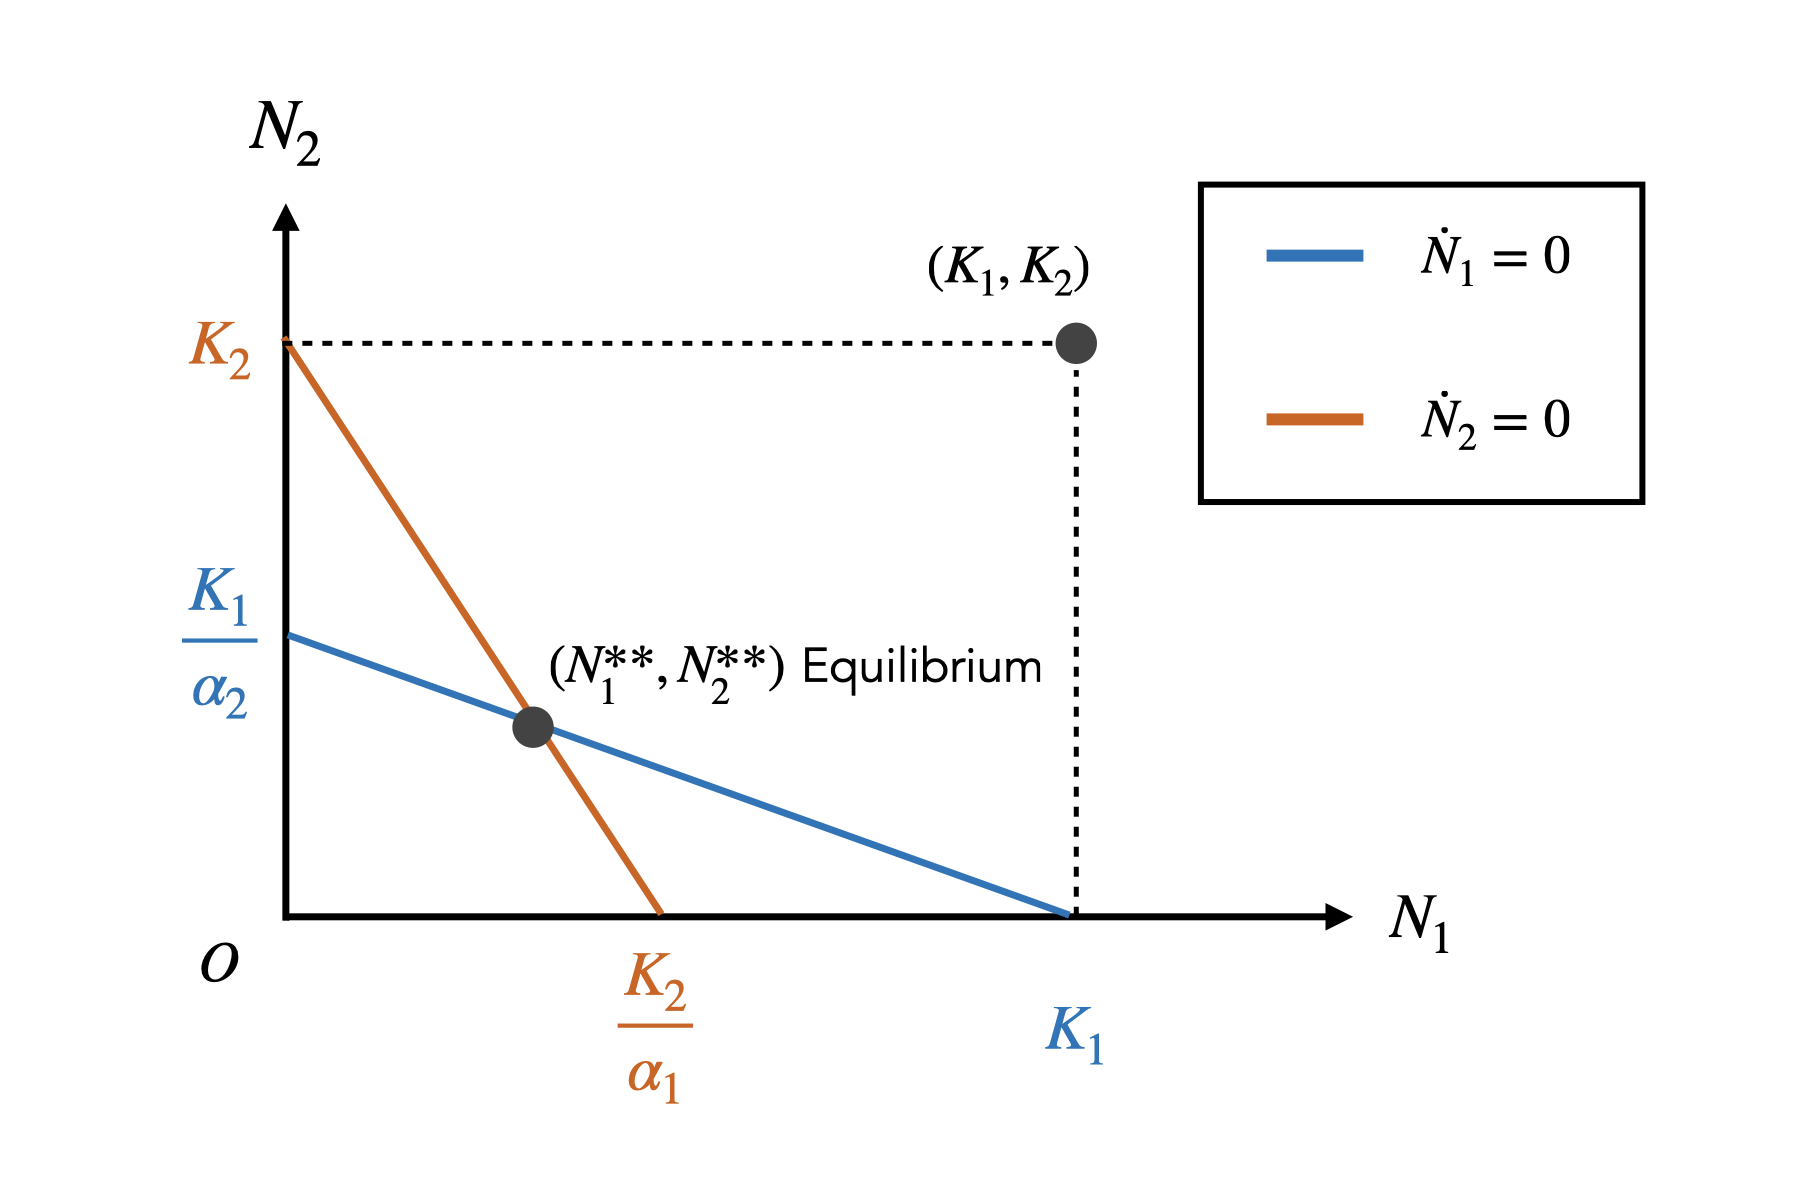
\includegraphics[width = \textwidth]{fig/graph_001.png}
  \caption {Nullclines for $N_1$ and $N_2$ and the equilibrium of the Lotka-Volterra system when Equation \ref{equ:constraints} is met.}
  \label{fig:graph_001}
\end{figure}

In determining the vector space, or rather the vectors' orientation on arbitrary points in the phase plane, we need a sample of a point on the phase plane. For simplicity, we take $(K_1, K_2)$.

Now we determine the orientation of the vector at $(K_1, K_2)$.
